%
% Recomendaciones del NIST para la generación de llaves,
% capítulo de análisis y diseño para la generación de tokens.
% Proyecto Lovelace.
%

\subsubsection{Generación de llaves}
\label{sec:generacion_llaves}

% NIST 800-133 ---

\textbf{Métodos para la generación de llaves}
La generación de llaves se puede hacer por medio del uso de generadores de 
bits aleatorios (\gls{gl:rbg}), de la derivación de llaves a partir de otras, 
de la derivación de llaves a partir de una contraseña, y del uso de un esquema 
de acuerdo entre llaves o \textit{key agreement}; pero todas, de forma directa 
o indirecta deben estar basadas en la salida de un \gls{gl:rbg}.

\textbf{Donde generar las llaves}
La generación de llaves criptográficas debe ir de acuerdo con el \gls{gl:fips} 
140 (descrito en \cite{nist_modulos_criptograficos}), y si es necesario que 
las llaves sean transferidas, se debe de hacer por medio de un canal seguro. 
Además, todos los valores aleatorio requeridos para la generación de las 
llaves deben ser generados dentro de un mismo módulo criptográfico.

\textbf{Fuerza de la seguridad}
Se dice que un método soporta la fuerza de seguridad, si la fuerza de 
seguridad provista por dicho método es igual o mayor a la seguridad 
requerida para la protección de la información.
\begin{itemize}

  \item La fuerza de seguridad para los \gls{gl:rbg} está basada en la 
    entropía o aleatoriedad que provee el mismo \gls{gl:rbg}.

  \item La seguridad de un algoritmo criptográfico se basa en el hecho de que 
  las llaves que usan fueron generadas usando procesos que las proveían de 
  una entropía mayor o igual a la necesaria para el algoritmo, así como el 
  mismo tamaño de la llave.

  \item La fuerza de seguridad de una llave depende de: el algoritmo que la 
  utilizara, su tamaño, el proceso con el que fue generada, y la forma en la 
  que es utilizada la llave.

\end{itemize}

\textbf{Usos de las salidas de los \gls{gl:rbg}}
Suponiendo que $K$ es una llave simétrica o un valor aleatorio que sirve 
como entrada de un algoritmo generador de pares de llaves asimétricas, $K$ 
debe ser una cadena de bit tal que: 

\begin{equation}
  \label{bits_K}
  K\: =\: U\: \oplus\: V
\end{equation}

donde $U$ es una cadena de bit que se obtuvo de un \gls{gl:rbg} con el 
soporte de fuerza de seguridad requerida, y $V$ es una cadena de bit de la 
misma longitud, que además fue generada de manera tal que es independiente de 
$U$ y viceversa. La independencia entre $U$ y $V$ se requiere debido a que se 
tiene que evitar que el conocimiento de alguno de estos valores no pueda 
usarse para obtener información del otro.

\textbf{Generación de pares de llaves asimétricas}
Los pares de llaves solo pueden ser generados o por el propietario del las 
mismas llaves, o por un tercero de confianza capaz de proveerlas.

Las llaves privadas debe permanecer secreta dentro del modulo criptográfico 
del propietario o de un tercero de confianza, además de que, si se tienen que 
transferir dichas llaves, se debe de garantizar que solo el propietario o la 
parte generadora pueden verlas en claro.

\textbf{Generación de llaves simétricas}
Las llaves deben de ser generadas por una o varias de las entidades que 
compartirán la llave, o por un tercero de confianza capaz compartirlas de una 
manera segura. 

Las llaves que son generadas directamente de un \gls{gl:rbg} deben de cumplir 
con la forma establecida en la ecuación \ref{bits_K}.

Cuando sea necesario compartir las llaves, su distribución debe de ser manual, 
o por medio de un envolvimiento de la llave o \textit{key wrapping}, el cual 
debe de soportar la fuerza de seguridad requerida para la protección de la 
información que protege la llave.

Obtener llaves derivadas de una contraseña es una práctica cuestionable, 
debido a que comúnmente la aleatoriedad en las contraseñas es mínima, por tal 
razón al generarse llaves de esta manera, es fuertemente recomendado que los 
usuarios selecciones contraseñas con una gran cantidad de entropía. De 
cualquier manera, se considera que este tipo de llaves proveen una entropía 
nula, a menos que la contraseña haya sido generada con un \gls{gl:rbg}.

Cuando se tiene un conjunto de llaves $K_1, \dots, K_n$ generadas de forma 
independiente, estas pueden ser combinadas entre sí para formar una llave $K$. 
Igualmente, si se tiene un conjunto de bloques de información $V_1, \dots, 
V_m$ que son independientes de sus respectivas llaves, se pueden combinar 
estos bloques y sus llaves para formar otra llave. 

Los métodos aprobados para generar llaves a partir de la combinación de 
otras son: 
\begin{itemize}

  \item La concatenación de varias llaves.

  $K\: =\: K_1\: \parallel\: \dots\: \parallel\: K_n$.

  \item La aplicación de compuertas \textit{xor} (o exclusiva) a varias llaves.

  $K\: =\: K_1\: \oplus\: \dots\: \oplus\: K_n$.
  
  \item La aplicación de compuertas \textit{xor} (o exclusiva) a varias llaves 
  y bloques de información.

  $K\: =\: K_1\: \oplus\: \dots\: \oplus\: K_n\: 
  \oplus\: V_1\: \oplus\: \dots\: \oplus\: V_m$.

\end{itemize}

Cuando sea necesario reemplazar una llave, la nueva llave debe de ser 
completamente independiente de la anterior, para que el conocimiento de esta 
ultima, no proporcione ningún conocimiento de la nueva.

% NIST 800-108 ---

\paragraph{Funciones Pseudoaleatorias (PRF)}

Las funciones pseudoaleatorias o \gls{gl:prf} son funciones computables en 
tiempo polinomial con un índice o semilla $s$ y una variable de entrada $x$, 
de manera que cuando $s$ se selecciona aleatoriamente de $S$, es 
computacionalmente indistinguible de una función aleatoria definida en el 
mismo dominio y rango que $PRF(s,x)$.

Cuando una llave criptográfica $K_I$ se usa como la semilla de una 
\gls{gl:prf}, la salida de la función pseudoaleatoria se puede utilizar 
cómo \gls{gl:material_llaves}.

Para la derivación de llaves se tiene permitido el uso de \gls{gl:hmac} o 
de \gls{gl:cmac} como la función pseudoaleatoria.

\paragraph{Funciones de derivación de llaves (KDF)}
Las funciones de derivación de llaves o \gls{gl:kdf} son funciones que a 
partir de una llave dada como entrada, son usadas para generar 
\gls{gl:material_llaves} capaz de ser empleado por varios algoritmos 
criptográficos. 

Las llaves de entradas de este tipo de funciones son llamadas \textit{key 
derivation key} y debe ser llaves criptográficas generadas por medio de un 
\gls{gl:rbg} o por un proceso automático de establecimiento de llaves.

El \gls{gl:material_llaves} segmentado es usado como llaves criptográficas 
correspondientes a distintos algoritmos que ofrecen diferentes servicios, por 
lo tanto las \gls{gl:kdf} deben de definir una manera de transformar este 
material en llaves distintas.

De forma general las \gls{gl:kdf} funcionan iterando $n$ veces funciones 
pseudoaleatoria para concatenar sus salidas hasta que se alcance la longitud 
de bits del \gls{gl:material_llaves}.

\paragraph{Modos de iteración}

Algo necesario para el funcionamiento de las \gls{gl:kdf} son los modo de 
iteración, que define las entradas que se tendrán, y el orden de los campos 
de salida en cada ciclo.

\textbf{Counter mode}
En la figura \ref{diagrama_counter_mode} se aprecia la forma de operación de 
este modo de iteración, en el que los datos de entrada son una cadena binaria 
de la forma: $Label \parallel 0x00 \parallel Context \parallel {[L]}_2$ 
donde el $Label$ es un valor que identifica el propósito del 
\gls{gl:material_llaves}, $0x00$ es un octeto de ceros, el $Context$ es una 
cadena con la información relacionada al \gls{gl:material_llaves}, y 
${[L]}_2$ es la longitud del \gls{gl:material_llaves} que se desea obtener.
Como se observa, en este modo de iteración el contador es parte la las 
entradas a la \gls{gl:prf}.

\begin{figure}[H]
  \begin{center}
    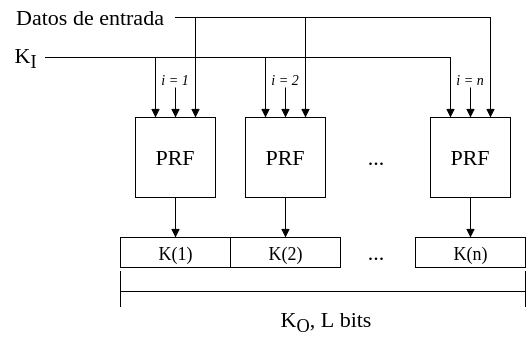
\includegraphics[width=0.75\linewidth]{diagramas/counter_mode}
    \caption{Diagrama del \textit{counter mode}.}
    \label{diagrama_counter_mode}
   \end{center}
\end{figure}

%Pseudocodigo excediéndose de los 80 para una correcta visualización el en pdf
\begin{pseudocodigo}[caption={Funcionamiento del \textit{counter mode}.}, 
label={mi:1}]
  entrada:   La llave $K_I$, la longitud $L$ y los valores de $Label$ y $Context$.
  salida:    $K_O$, con una longitud de $L$ bits.
  inicio
    calcular $n\: =\: [\frac{L}{h}]$, donde $h$ es la longitud de salida de la $PRF$.
    si $n$ > $2^r-1$, indicar error y parar; donde $r\: \leq\: 32$.
    $resultado(0) = \emptyset$
    para $i=1$ hasta $n$:
      $K(i)\: =\: PRF(K_I,\: {[i]}_2 \parallel Label \parallel 0x00 \parallel Context \parallel {[L]}_2 )$.
      $resultado(i)\: =\: resultado(i-1) \parallel K(i)$.
    $K_O =$ los L bits más a la izquierda del $resultado(n)$.
  fin
\end{pseudocodigo}

\textbf{Feedback mode}
Este modo de iteración opera tomando las salidas la \gls{gl:prf} en 
iteraciones pasadas, como parte de las entradas de la iteración actual.
Cabe resaltar que como se muestra en la figura \ref{diagrama_feedback_mode}, 
es opcional tener un contador concatenado a los datos de entrada, e igualmente 
los datos de entrada son como en el modo de operación anterior, solo que con 
un vector de inicialización $IV$.

\begin{figure}[H]
  \begin{center}
    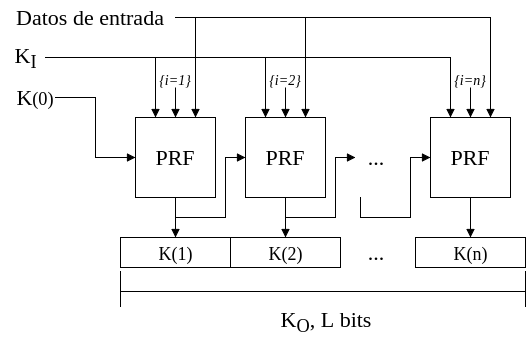
\includegraphics[width=0.75\linewidth]{diagramas/feedback_mode}
    \caption{Diagrama del \textit{feedback mode}.}
    \label{diagrama_feedback_mode}
   \end{center}
\end{figure}

%Pseudocodigo excediéndose de los 80 para una correcta visualización el en pdf
\begin{pseudocodigo}[caption={Funcionamiento del \textit{feedback mode}.}, 
label={mi:2}]
  entrada:   La llave $K_I$, la longitud $L$, el vector de inicialización IV 
             y los valores de $Label$ y $Context$.
  salida:    $K_O$, con una longitud de $L$ bits.
  inicio
    calcular $n\: =\: [\frac{L}{h}]$, donde $h$ es la longitud de salida de la $PRF$.
    si $n$ > $2^{32}-1$, indicar error y parar.
    $resultado(0)\: =\: \emptyset$.
    $K(0) = IV$.
    para $i=1$ hasta $n$:
      $K(i)\: = \:PRF(K_I,\: K(i-1)\: \{\parallel {[i]}_2\}\: \parallel Label \parallel 0x00 \parallel Context \parallel {[L]}_2 )$.
      $resultado(i)\: =\: resultado(i-1) \parallel K(i)$.
    $K_O =$ los L bits más a la izquierda del $resultado(n)$. 
  fin
\end{pseudocodigo}

\textbf{Double pipeline mode}
Como su nombre lo indica y a diferencia de los otros dos modos de iteración 
mencionados, este usa dos flujos, donde un flujo está encargado de generar 
valores secretos, y el otro usa como entradas las salidas del primero.
Los valores de entrada son iguales que en el primer modo de iteración descrito, 
y su funcionamiento está descrito en la figura \ref{diagrama_dpipeline_mode}.

\begin{figure}[H]
  \begin{center}
    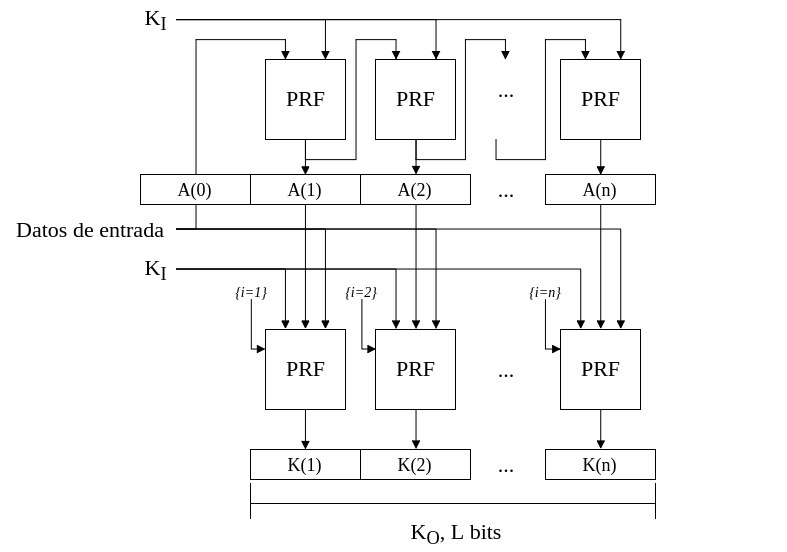
\includegraphics[width=0.75\linewidth]{diagramas/dpipeline_mode}
    \caption{Diagrama del \textit{double pipeline mode}.}
    \label{diagrama_dpipeline_mode}
   \end{center}
\end{figure}

%Pseudocodigo excediéndose de los 80 para una correcta visualización el en pdf
\begin{pseudocodigo}[caption={Funcionamiento del \textit{double pipeline mode}.}, 
label={mi:3}]
  entrada:   La llave $K_I$, la longitud $L$ y los valores de $Label$ y $Context$.
  salida:    $K_O$, con una longitud de $L$ bits.
  inicio
    calcular $n\: =\: [\frac{L}{h}]$, donde $h$ es la longitud de salida de la PRF.
    si $n$ > $2^{32}-1$, indicar error y parar.
    $resultado(0)\: =\: \emptyset$.
    $A(0)\: =\: IV\: =\: Label \parallel 0x00 \parallel Context \parallel {[L]}_2$
    para $i=1$ hasta $n$:
      $A(i)\: =\: PRF(K_I, A(i-1))$.
      $K(i)\: =\: PRF(K_I,\: A(i)\: \{\parallel {[i]}_2\}\: \parallel Label \parallel 0x00 \parallel Context \parallel {[L]}_2)$.
      $resultado(i) = resultado(i-1) \parallel K(i)$.
    $K_O =$ los L bits más a la izquierda del $resultado(n)$. 
  fin
\end{pseudocodigo}

\textbf{Jerarquía de llaves}
El \gls{gl:material_llaves} proveniente de una derivación puede ser usado una 
o más veces como llave de entrada de otras derivaciones subsecuentes, así, es 
posible establecer una jerarquía en la que las llaves tienen distintos niveles.

\paragraph{Consideraciones de seguridad\newline}

\textbf{Fuerza criptográfica}
La fuerza de seguridad de una \gls{gl:kdf} es medida por la cantidad de 
trabajo requerido para distinguir su cadena de salida de una cadena de bits 
que en verdad es uniformemente distribuida y de la misma longitud, suponiendo 
que la llave de entrada $K_I$, es la única entrada desconocida para la 
\gls{gl:kdf}.

\textbf{La longitud de la llave de entrada}
En algunas \gls{gl:kdf} el tamaño de la llave $K_I$ está definido por la 
\gls{gl:prf} que usa internamente, por ejemplo cuando se usa \gls{gl:cmac}, 
pero igualmente, otras \gls{gl:kdf} pueden usar llaves de cualquier tamaño, 
como al usar \gls{gl:hmac} como \gls{gl:prf}.

\textbf{Transformación de material de llaves a llaves criptográficas}
La longitud $L$ del material de llaves está limitado tanto por el algoritmo 
que relacionado a la salida del \gls{gl:kdf}, como por el modo de iteración 
que se usa.

\textbf{Codificación de los datos de entrada}
La información de entrada de una \gls{gl:kdf} consiste en diferentes campos 
de datos, estos deben de estar ordenados de forma específica y sin ambigüedad, 
de forma que se tenga un método de codificación capaz de mapear uno a uno cada 
campo. Esto es necesario para poder detectar ataques en el \gls{gl:kdf} que 
dependan de la manipulación de esta información.

\textbf{Separación entre llaves}
Las llaves provenientes del \gls{gl:material_llaves} deben de estar separadas 
criptográficamente, de tal manera que no se comprometa la seguridad de ninguna 
de estas llaves derivadas. Cuando el \gls{gl:material_llaves} se obtiene de 
múltiples ejecuciones del \gls{gl:kdf} usando la misma llave de entrada $K_I$, 
el \gls{gl:kdf} debe de garantizar que el \gls{gl:material_llaves} de una 
ejecución no comprometa al de cualquier otra.

\textbf{Enlace de contexto}
Todo el \gls{gl:material_llaves} debe estar ligado a todas las entidades 
relacionadas para poder evitar errores de protocolo.

